\documentclass[../main/journal_template.tex]{subfiles}
% This ties 

\begin{document}


\section{Electrodynamics}\label{sec:physics_electrodyn}
% Note: You can label things locally, but referencing labels in *other* subfiles will only show up in the main document
From Jackson \cite{jackson1999classical}: 



\section{Figures}
To include images, you can put them anywhere in the folder structure, but you have to give an absolute path relative to the base folder.  For instance, in the folder \verb|figures|, there is a picture called \verb|LIGO.png|.  However, to include this image, I must use \verb|../physics/figures/LIGO.png| i.e. I have to go up to the main folder then back down.  This is so the main file will know where this image is.

\begin{figure}[ht]
\begin{center}
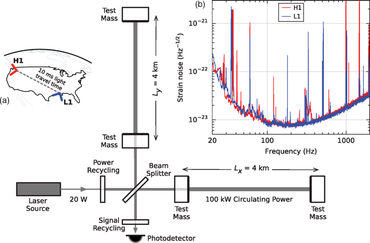
\includegraphics[scale=1]{../physics/figures/LIGO.png}
\end{center}
\caption{A figure about the LIGO gravity wave detector}
\label{somefig}
\end{figure}



\begin{comment}
\bibliographystyle{plain}
\bibliography{../main/journal_template_bib}
\end{comment}
\printbib{../main/journal_template_bib}

\end{document}